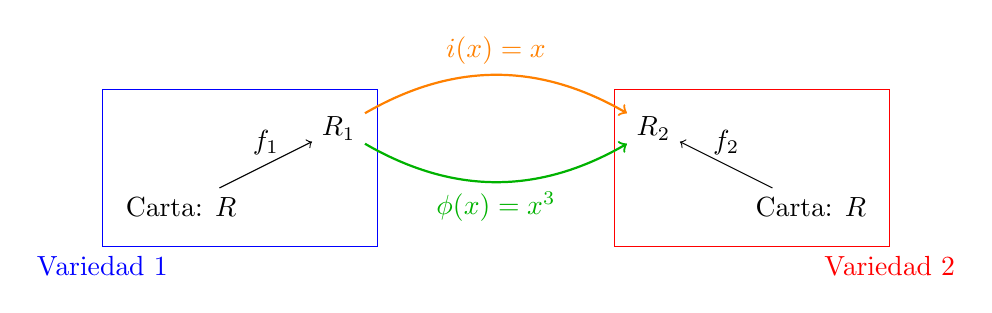
\begin{tikzpicture}
\begin{scope}
\node (R-a) at (0,0) {Carta: $\mathbb{R}$};
\node (R-1) at (2, 1) {$\mathbb{R}_1$};
\draw[->] (R-a) -- node[midway, above] {$f_1$} (R-1);
\draw[blue] (-1, -0.5) node[below] {Variedad 1} rectangle (2.5, 1.5);
\end{scope}

\begin{scope}[xshift=8cm]
\node (R-b) at (0,0) {Carta: $\mathbb{R}$};
\node (R-2) at (-2, 1) {$\mathbb{R}_2$};
\draw[->] (R-b) -- node[midway, above] {$f_2$} (R-2);
\draw[red] (1, -0.5) node [below] {Variedad 2} rectangle (-2.5, 1.5);
\end{scope}

\draw[thick, orange, ->] (R-1) to[bend left] node[midway, above] {$i(x) = x$} (R-2);
\draw[thick, green!70!black, ->] (R-1) to[bend right] node[midway, below] {$\phi(x) = x^3$} (R-2);
\end{tikzpicture}
